\section{Cost Budget Breakdown}
\label{blBudgetCost}
For a preliminary estimation of cost breakdown it is necessary to realize the different stages of the life-cycle costs. These are the costs of the entire space mission from the first stages of planning until end of life.
%
%\begin{wrapfigure}{L}{1\textwidth}[H]
%	\begin{center}
%  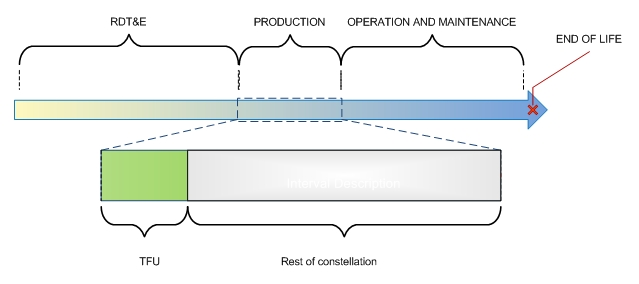
\includegraphics[width=1\textwidth]{chapters/img/lifetime.jpg}
%  \end{center}
%  \caption{Life-Cycle}
%  \label{fig:lifecycle}
%\end{wrapfigure}

\begin{figure}[b]
\begin{center}

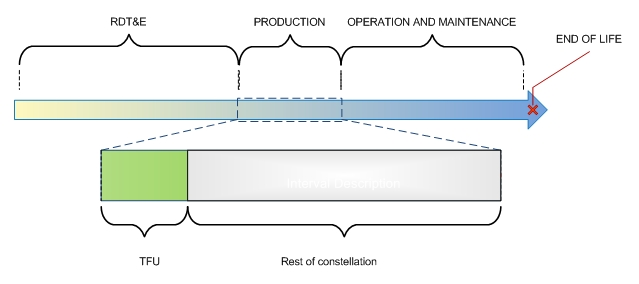
\includegraphics[width=0.7\textwidth]{chapters/img/lifetime.jpg}
\caption{Life-Cycle}
\label{fig:lifecycle}
\end{center}
\end{figure}

Figure \ref{fig:lifecycle} shows a typical life-cycle for a space mission. The \ac{RDTE} stage includes the planning, development and testing of all prototypes and qualification units, but does not include the technology development for different subsystems. In the case of the laser swarm this is largely dependent on the single emitter and one receiver unit. This stage is also mostly consistent of non-recurring costs. The production stage consists of actual manufacture of the physical satellites. The cost estimation in this stage is based on the \ac{TFU}. This is done because it is assumed that the first unit (in the case of the Laser Swarm, that would be the emitter and one receiver) would be the most expensive to produce. The rest of the swarm constellation satellite costs are calculated by taking a theoretical learning curve\cite{larson}. 

The final stage - \ac{OM} is self explanatory. This phase can be very expensive for large constellations. The ground segment is the prevailing factor.

The cost breakdown can be found in figure \ref{fig:costbreak} on page \pageref{fig:costbreak}. In this diagram, the cost is broken down into segments. This way it is easier to follow cost distribution down to all subsystems.

Because of the nature of the system that is being designed - as a collection of satellites, it is very hard to make an accurate prediction of costs before critical decisions have been made. Most subsystem costs are mass driven, so design options create a large margin of error at early estimations. Furthermore, due to high cost of actual production of individual satellites, a swarm is hard to predict without a rough idea of the number of space platforms. It is important to note that cost is also dependent on so called heritage factors. These factors allow for reduction of costs based on already existing designs. However, if some kind of new technology is used in a subsystem then this reduction cannot be used.

Table \ref{tab:CostBreakdown} on page \pageref{tab:CostBreakdown} contains percentage estimations of all aspects covered in figure \ref{fig:costbreak}.

\begin{figure}[H]
\begin{center}

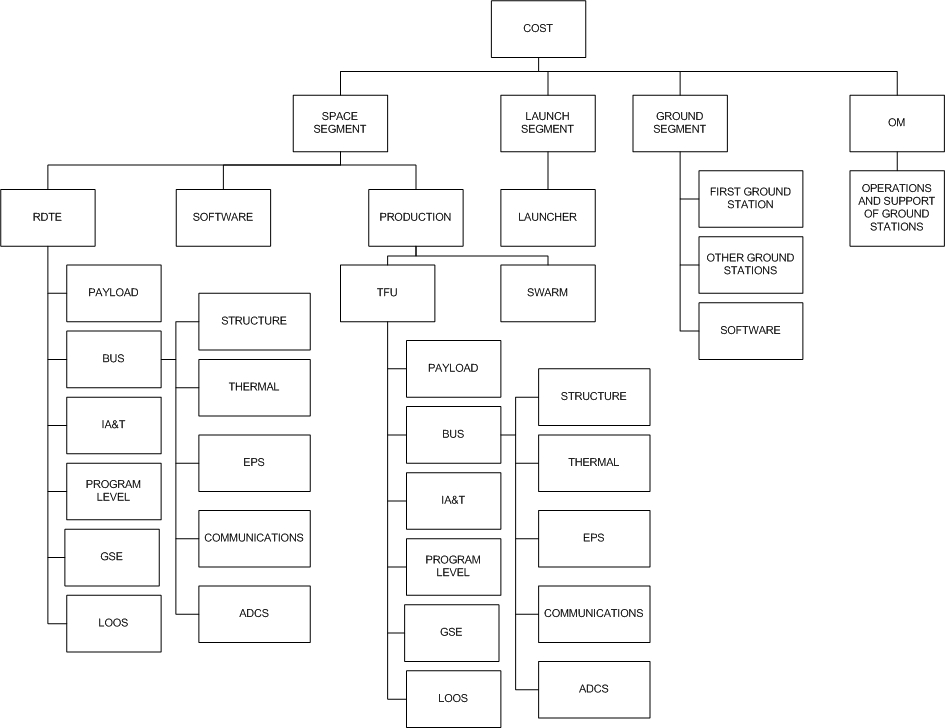
\includegraphics[width=1.0\textwidth,angle=90]{chapters/img/costbreakdown.jpg}
\caption{Cost breakdown}
\label{fig:costbreak}
\end{center}
\end{figure}

\begin{table*}[htbp]
	\centering

% Table generated by Excel2LaTeX from sheet 'Sheet1'
\begin{tabular}{p{10cm} | c | c }

   \textbf{SEGMENT} & \textbf{\% OF PARENT} & \textbf{\% OF TOTAL} \\ \hline \hline

\textsl{Space Segment} &          &       30   \\ \hline

      \hspace{1.0cm}RDTE &         30 &   9       \\ \hline

   \hspace{2.0cm}Payload &         26 &     2.3     \\

       \hspace{2.0cm}Bus &         52 &     4.7    \\ \hline

 \hspace{2.5cm}Structure &         24&      1.1    \\

  \hspace{2.5cm}Thermal &         2 &       0.1   \\

      \hspace{2.5cm}EPS &         22 &      1    \\

\hspace{2.5cm}Communications &         38 &      1.8    \\

      \hspace{2.5cm}ADCS &         14 &     0.7     \\ \hline

       \hspace{2.0cm}IAT &         0 &         0 \\

 \hspace{2.0cm}Program Level &         22 &       2   \\ \hline
 \hspace{2.5cm}Program Management &         20 &      0.4    \\
 \hspace{2.5cm}Systems Engineering &         40 &     0.8     \\
 \hspace{2.5cm}Product Assurance &         20 &       0.4   \\
 \hspace{2.5cm}System Evaluation &         20 &       0.4   \\ \hline

        \hspace{2.0cm}GSE &         4 &      0.4    \\

      \hspace{2.0cm}LOOS &         0 &         0 \\ \hline

  \hspace{1.0cm}Software &         25 &         7.5 \\

\hspace{1.0cm}Production &         45 &         13.5 \\ \hline

       \hspace{2.0cm}TFU &         10-30 &       1.4-4.8   \\ \hline

   \hspace{2.5cm}Payload &         20 &       0.3-0.8   \\

       \hspace{2.5cm}Bus &         45 &        0.6-1.8  \\ \hline

 \hspace{3.0cm}Structures &         24 &       0.1-0.4   \\

   \hspace{3.0cm}Thermal &         5 &         0.04-0.12 \\

       \hspace{3.0cm}EPS &         20 &        0.1-0.4  \\

\hspace{3.0cm}Communications &         18 &      0.1-0.3    \\

      \hspace{3.0cm}ADCS &         28 &         0.2-0.5 \\ \hline

       \hspace{2.5cm}IAT &         14&         0.2-0.6 \\

\hspace{2.5cm}Program Level &         13 &         0.2-0.5 \\ \hline
 \hspace{3.0cm}Program Management &         30 &       0.05-0.16   \\
 \hspace{3.0cm}Systems Engineering &         20 &        0.04-0.11  \\
 \hspace{3.0cm}Product Assurance &         30 &       0.05-0.16   \\
 \hspace{3.0cm}System Evaluation &         20 &       0.04-0.11   \\ \hline

       \hspace{2.5cm}GSE &         0 &          0\\

      \hspace{2.5cm}LOOS &         5 &         0.07-0.2 \\ \hline

     \hspace{2.0cm}Swarm &         70-90 &         9.5-12 \\ \hline

\textit{Launch Segment} &         &         5-10 \\ \hline

  \hspace{1.0cm}Launcher &         100 &        5-10  \\ \hline

\textit{Ground Segment} &          &     20     \\ \hline

\hspace{1.0cm}First Ground Station &         25 &      5    \\

\hspace{1.0cm}Consecutive Ground Stations &         55 &     11     \\

\hspace{1.0cm}Software &         20 &     4     \\ \hline

\textit{Operations and Maintenance} &          &        45  \\ \hline

\hspace{1.0cm}Operations and support of ground stations &         100 &   45       \\
	
\end{tabular} 
\caption{Cost Breakdown}
	\label{tab:CostBreakdown} 
\end{table*}



